% Generated by Sphinx.
\def\sphinxdocclass{report}
\documentclass[letterpaper,10pt,english]{sphinxmanual}
\usepackage[utf8]{inputenc}
\DeclareUnicodeCharacter{00A0}{\nobreakspace}
\usepackage{cmap}
\usepackage[T1]{fontenc}
\usepackage{babel}
\usepackage{times}
\usepackage[Bjarne]{fncychap}
\usepackage{longtable}
\usepackage{sphinx}
\usepackage{multirow}


\title{PoissonFEM Documentation}
\date{October 13, 2013}
\release{1.0.0}
\author{Rafał Białozor}
\newcommand{\sphinxlogo}{}
\renewcommand{\releasename}{Release}
\makeindex

\makeatletter
\def\PYG@reset{\let\PYG@it=\relax \let\PYG@bf=\relax%
    \let\PYG@ul=\relax \let\PYG@tc=\relax%
    \let\PYG@bc=\relax \let\PYG@ff=\relax}
\def\PYG@tok#1{\csname PYG@tok@#1\endcsname}
\def\PYG@toks#1+{\ifx\relax#1\empty\else%
    \PYG@tok{#1}\expandafter\PYG@toks\fi}
\def\PYG@do#1{\PYG@bc{\PYG@tc{\PYG@ul{%
    \PYG@it{\PYG@bf{\PYG@ff{#1}}}}}}}
\def\PYG#1#2{\PYG@reset\PYG@toks#1+\relax+\PYG@do{#2}}

\def\PYG@tok@gd{\def\PYG@tc##1{\textcolor[rgb]{0.63,0.00,0.00}{##1}}}
\def\PYG@tok@gu{\let\PYG@bf=\textbf\def\PYG@tc##1{\textcolor[rgb]{0.50,0.00,0.50}{##1}}}
\def\PYG@tok@gt{\def\PYG@tc##1{\textcolor[rgb]{0.00,0.25,0.82}{##1}}}
\def\PYG@tok@gs{\let\PYG@bf=\textbf}
\def\PYG@tok@gr{\def\PYG@tc##1{\textcolor[rgb]{1.00,0.00,0.00}{##1}}}
\def\PYG@tok@cm{\let\PYG@it=\textit\def\PYG@tc##1{\textcolor[rgb]{0.25,0.50,0.56}{##1}}}
\def\PYG@tok@vg{\def\PYG@tc##1{\textcolor[rgb]{0.73,0.38,0.84}{##1}}}
\def\PYG@tok@m{\def\PYG@tc##1{\textcolor[rgb]{0.13,0.50,0.31}{##1}}}
\def\PYG@tok@mh{\def\PYG@tc##1{\textcolor[rgb]{0.13,0.50,0.31}{##1}}}
\def\PYG@tok@cs{\def\PYG@tc##1{\textcolor[rgb]{0.25,0.50,0.56}{##1}}\def\PYG@bc##1{\colorbox[rgb]{1.00,0.94,0.94}{##1}}}
\def\PYG@tok@ge{\let\PYG@it=\textit}
\def\PYG@tok@vc{\def\PYG@tc##1{\textcolor[rgb]{0.73,0.38,0.84}{##1}}}
\def\PYG@tok@il{\def\PYG@tc##1{\textcolor[rgb]{0.13,0.50,0.31}{##1}}}
\def\PYG@tok@go{\def\PYG@tc##1{\textcolor[rgb]{0.19,0.19,0.19}{##1}}}
\def\PYG@tok@cp{\def\PYG@tc##1{\textcolor[rgb]{0.00,0.44,0.13}{##1}}}
\def\PYG@tok@gi{\def\PYG@tc##1{\textcolor[rgb]{0.00,0.63,0.00}{##1}}}
\def\PYG@tok@gh{\let\PYG@bf=\textbf\def\PYG@tc##1{\textcolor[rgb]{0.00,0.00,0.50}{##1}}}
\def\PYG@tok@ni{\let\PYG@bf=\textbf\def\PYG@tc##1{\textcolor[rgb]{0.84,0.33,0.22}{##1}}}
\def\PYG@tok@nl{\let\PYG@bf=\textbf\def\PYG@tc##1{\textcolor[rgb]{0.00,0.13,0.44}{##1}}}
\def\PYG@tok@nn{\let\PYG@bf=\textbf\def\PYG@tc##1{\textcolor[rgb]{0.05,0.52,0.71}{##1}}}
\def\PYG@tok@no{\def\PYG@tc##1{\textcolor[rgb]{0.38,0.68,0.84}{##1}}}
\def\PYG@tok@na{\def\PYG@tc##1{\textcolor[rgb]{0.25,0.44,0.63}{##1}}}
\def\PYG@tok@nb{\def\PYG@tc##1{\textcolor[rgb]{0.00,0.44,0.13}{##1}}}
\def\PYG@tok@nc{\let\PYG@bf=\textbf\def\PYG@tc##1{\textcolor[rgb]{0.05,0.52,0.71}{##1}}}
\def\PYG@tok@nd{\let\PYG@bf=\textbf\def\PYG@tc##1{\textcolor[rgb]{0.33,0.33,0.33}{##1}}}
\def\PYG@tok@ne{\def\PYG@tc##1{\textcolor[rgb]{0.00,0.44,0.13}{##1}}}
\def\PYG@tok@nf{\def\PYG@tc##1{\textcolor[rgb]{0.02,0.16,0.49}{##1}}}
\def\PYG@tok@si{\let\PYG@it=\textit\def\PYG@tc##1{\textcolor[rgb]{0.44,0.63,0.82}{##1}}}
\def\PYG@tok@s2{\def\PYG@tc##1{\textcolor[rgb]{0.25,0.44,0.63}{##1}}}
\def\PYG@tok@vi{\def\PYG@tc##1{\textcolor[rgb]{0.73,0.38,0.84}{##1}}}
\def\PYG@tok@nt{\let\PYG@bf=\textbf\def\PYG@tc##1{\textcolor[rgb]{0.02,0.16,0.45}{##1}}}
\def\PYG@tok@nv{\def\PYG@tc##1{\textcolor[rgb]{0.73,0.38,0.84}{##1}}}
\def\PYG@tok@s1{\def\PYG@tc##1{\textcolor[rgb]{0.25,0.44,0.63}{##1}}}
\def\PYG@tok@gp{\let\PYG@bf=\textbf\def\PYG@tc##1{\textcolor[rgb]{0.78,0.36,0.04}{##1}}}
\def\PYG@tok@sh{\def\PYG@tc##1{\textcolor[rgb]{0.25,0.44,0.63}{##1}}}
\def\PYG@tok@ow{\let\PYG@bf=\textbf\def\PYG@tc##1{\textcolor[rgb]{0.00,0.44,0.13}{##1}}}
\def\PYG@tok@sx{\def\PYG@tc##1{\textcolor[rgb]{0.78,0.36,0.04}{##1}}}
\def\PYG@tok@bp{\def\PYG@tc##1{\textcolor[rgb]{0.00,0.44,0.13}{##1}}}
\def\PYG@tok@c1{\let\PYG@it=\textit\def\PYG@tc##1{\textcolor[rgb]{0.25,0.50,0.56}{##1}}}
\def\PYG@tok@kc{\let\PYG@bf=\textbf\def\PYG@tc##1{\textcolor[rgb]{0.00,0.44,0.13}{##1}}}
\def\PYG@tok@c{\let\PYG@it=\textit\def\PYG@tc##1{\textcolor[rgb]{0.25,0.50,0.56}{##1}}}
\def\PYG@tok@mf{\def\PYG@tc##1{\textcolor[rgb]{0.13,0.50,0.31}{##1}}}
\def\PYG@tok@err{\def\PYG@bc##1{\fcolorbox[rgb]{1.00,0.00,0.00}{1,1,1}{##1}}}
\def\PYG@tok@kd{\let\PYG@bf=\textbf\def\PYG@tc##1{\textcolor[rgb]{0.00,0.44,0.13}{##1}}}
\def\PYG@tok@ss{\def\PYG@tc##1{\textcolor[rgb]{0.32,0.47,0.09}{##1}}}
\def\PYG@tok@sr{\def\PYG@tc##1{\textcolor[rgb]{0.14,0.33,0.53}{##1}}}
\def\PYG@tok@mo{\def\PYG@tc##1{\textcolor[rgb]{0.13,0.50,0.31}{##1}}}
\def\PYG@tok@mi{\def\PYG@tc##1{\textcolor[rgb]{0.13,0.50,0.31}{##1}}}
\def\PYG@tok@kn{\let\PYG@bf=\textbf\def\PYG@tc##1{\textcolor[rgb]{0.00,0.44,0.13}{##1}}}
\def\PYG@tok@o{\def\PYG@tc##1{\textcolor[rgb]{0.40,0.40,0.40}{##1}}}
\def\PYG@tok@kr{\let\PYG@bf=\textbf\def\PYG@tc##1{\textcolor[rgb]{0.00,0.44,0.13}{##1}}}
\def\PYG@tok@s{\def\PYG@tc##1{\textcolor[rgb]{0.25,0.44,0.63}{##1}}}
\def\PYG@tok@kp{\def\PYG@tc##1{\textcolor[rgb]{0.00,0.44,0.13}{##1}}}
\def\PYG@tok@w{\def\PYG@tc##1{\textcolor[rgb]{0.73,0.73,0.73}{##1}}}
\def\PYG@tok@kt{\def\PYG@tc##1{\textcolor[rgb]{0.56,0.13,0.00}{##1}}}
\def\PYG@tok@sc{\def\PYG@tc##1{\textcolor[rgb]{0.25,0.44,0.63}{##1}}}
\def\PYG@tok@sb{\def\PYG@tc##1{\textcolor[rgb]{0.25,0.44,0.63}{##1}}}
\def\PYG@tok@k{\let\PYG@bf=\textbf\def\PYG@tc##1{\textcolor[rgb]{0.00,0.44,0.13}{##1}}}
\def\PYG@tok@se{\let\PYG@bf=\textbf\def\PYG@tc##1{\textcolor[rgb]{0.25,0.44,0.63}{##1}}}
\def\PYG@tok@sd{\let\PYG@it=\textit\def\PYG@tc##1{\textcolor[rgb]{0.25,0.44,0.63}{##1}}}

\def\PYGZbs{\char`\\}
\def\PYGZus{\char`\_}
\def\PYGZob{\char`\{}
\def\PYGZcb{\char`\}}
\def\PYGZca{\char`\^}
\def\PYGZsh{\char`\#}
\def\PYGZpc{\char`\%}
\def\PYGZdl{\char`\$}
\def\PYGZti{\char`\~}
% for compatibility with earlier versions
\def\PYGZat{@}
\def\PYGZlb{[}
\def\PYGZrb{]}
\makeatother

\begin{document}

\maketitle
\tableofcontents
\phantomsection\label{index::doc}


Contents:


\chapter{Równanie Poissona:}
\label{index:rownanie-poissona}\label{index:rozwiazanie-rownania-poissona-metoda-elementow-skonczonych}
W ogólnym przypadku równanie Poissona ma postać:
\begin{gather}
\begin{split}\frac{\partial ^{2}}{\partial x^{2}} u(x,y,z)+
\frac{\partial ^{2}}{\partial y^{2}} u(x,y,z)+
\frac{\partial ^{2}}{\partial z^{2}} u(x,y,z) = f(x,y,z)\end{split}\notag\\\begin{split}\end{split}\notag
\end{gather}
lub zapisując krócej:
\begin{gather}
\begin{split}\nabla ^{2} u = f\end{split}\notag\\\begin{split}\end{split}\notag
\end{gather}

\chapter{Przykład 1}
\label{index:przyklad-1}
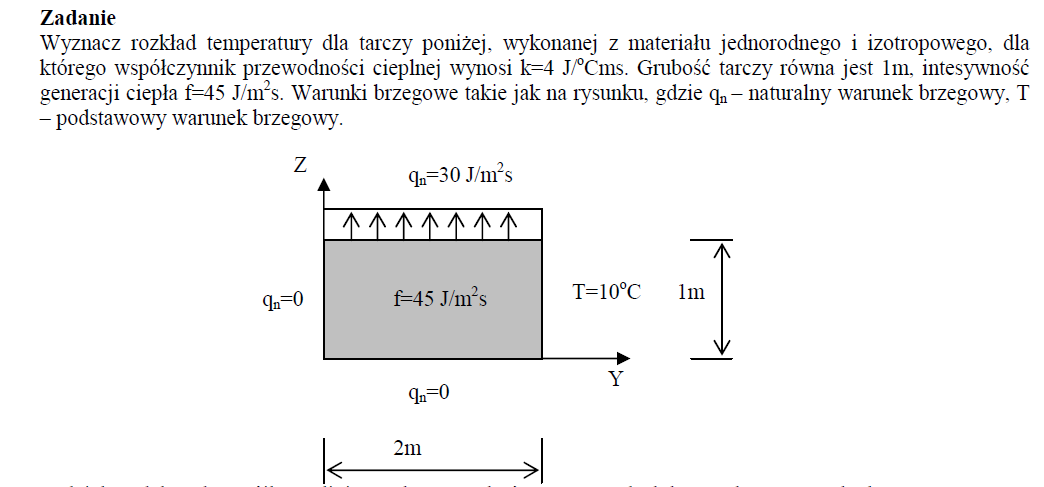
\includegraphics{zad.png}

Zdefiniujmy obszar w ktorym poszukiwać będziemy naszego rozwiązania.

\begin{Verbatim}[commandchars=\\\{\}]
\PYG{n+nb}{int} \PYG{n}{dlugosc}\PYG{o}{=}\PYG{l+m+mi}{2}\PYG{p}{,} \PYG{n}{wysokosc}\PYG{o}{=}\PYG{l+m+mi}{1}\PYG{p}{;}

\PYG{o}{/}\PYG{o}{/} \PYG{n}{Definicja} \PYG{n}{konturu}

\PYG{n+nb}{int} \PYG{n}{lewy}\PYG{o}{=}\PYG{l+m+mi}{1}\PYG{p}{;}
\PYG{n+nb}{int} \PYG{n}{dolny}\PYG{o}{=}\PYG{l+m+mi}{2}\PYG{p}{;}
\PYG{n+nb}{int} \PYG{n}{prawy}\PYG{o}{=}\PYG{l+m+mi}{3}\PYG{p}{;}
\PYG{n+nb}{int} \PYG{n}{gorny}\PYG{o}{=}\PYG{l+m+mi}{4}\PYG{p}{;}

\PYG{n}{border} \PYG{n}{left}\PYG{p}{(}\PYG{n}{t}\PYG{o}{=}\PYG{n}{wysokosc}\PYG{p}{,}\PYG{l+m+mi}{0}\PYG{p}{)} \PYG{p}{\PYGZob{}}\PYG{n}{x}\PYG{o}{=}\PYG{l+m+mi}{0}\PYG{p}{;} \PYG{n}{y}\PYG{o}{=}\PYG{n}{t}\PYG{p}{;}\PYG{n}{label}\PYG{o}{=}\PYG{n}{lewy}\PYG{p}{;}\PYG{p}{\PYGZcb{}}\PYG{p}{;}
\PYG{n}{border} \PYG{n}{bottom}\PYG{p}{(}\PYG{n}{t}\PYG{o}{=}\PYG{l+m+mi}{0}\PYG{p}{,}\PYG{n}{dlugosc}\PYG{p}{)} \PYG{p}{\PYGZob{}}\PYG{n}{x}\PYG{o}{=}\PYG{n}{t}\PYG{p}{;} \PYG{n}{y}\PYG{o}{=}\PYG{l+m+mi}{0}\PYG{p}{;}\PYG{n}{label}\PYG{o}{=}\PYG{n}{dolny}\PYG{p}{;}\PYG{p}{\PYGZcb{}}\PYG{p}{;}
\PYG{n}{border} \PYG{n}{right}\PYG{p}{(}\PYG{n}{t}\PYG{o}{=}\PYG{l+m+mi}{0}\PYG{p}{,}\PYG{n}{wysokosc}\PYG{p}{)} \PYG{p}{\PYGZob{}}\PYG{n}{x}\PYG{o}{=}\PYG{n}{dlugosc}\PYG{p}{;} \PYG{n}{y}\PYG{o}{=}\PYG{n}{t}\PYG{p}{;}\PYG{n}{label}\PYG{o}{=}\PYG{n}{prawy}\PYG{p}{;}\PYG{p}{\PYGZcb{}}\PYG{p}{;}
\PYG{n}{border} \PYG{n}{top}\PYG{p}{(}\PYG{n}{t}\PYG{o}{=}\PYG{n}{dlugosc}\PYG{p}{,}\PYG{l+m+mi}{0}\PYG{p}{)} \PYG{p}{\PYGZob{}}\PYG{n}{x}\PYG{o}{=}\PYG{n}{t}\PYG{p}{;} \PYG{n}{y}\PYG{o}{=}\PYG{n}{wysokosc}\PYG{p}{;}\PYG{n}{label}\PYG{o}{=}\PYG{n}{gorny}\PYG{p}{;}\PYG{p}{\PYGZcb{}}\PYG{p}{;}
\end{Verbatim}

Brzeg obszaru określa się przy użyciu funkcji parametrycznych $x=f(t)$ i $y=g(t)$.
Zdefiniowany brzeg zgodny jest z obiegiem w lewo. Definiowanie brzegów obszarów zgodnie z obiegiem,
jest istotną sprawą przy definiowaniu otworów w zadanym obszarze, tym problemem zajmiemy się jednak później.

Generowanie siatki trójkątnej.
Zdefiniujmy zmienne typu int określające liczbę węzłów zadanych na brzegach obszaru

\begin{Verbatim}[commandchars=\\\{\}]
\PYG{n+nb}{int} \PYG{n}{NpSzerokosc}\PYG{o}{=}\PYG{l+m+mi}{10} \PYG{p}{;}
\PYG{n+nb}{int} \PYG{n}{NpDlugosc}\PYG{o}{=}\PYG{l+m+mi}{10} \PYG{p}{;}

\PYG{n}{mesh} \PYG{n}{siatka}\PYG{o}{=}\PYG{n}{buildmesh}\PYG{p}{(}\PYG{n}{left}\PYG{p}{(}\PYG{n}{NpSzerokosc}\PYG{p}{)}\PYG{o}{+}\PYG{n}{top}\PYG{p}{(}\PYG{n}{NpDlugosc}\PYG{p}{)}
\PYG{o}{+}\PYG{n}{right}\PYG{p}{(}\PYG{n}{NpSzerokosc}\PYG{p}{)}\PYG{o}{+}\PYG{n}{bottom}\PYG{p}{(}\PYG{n}{NpDlugosc}\PYG{p}{)}\PYG{p}{)}\PYG{p}{;}
\end{Verbatim}

Podobnie jak w pythonie, wizualizację obiektów uzykujemy poleceniem \emph{plot}

\begin{Verbatim}[commandchars=\\\{\}]
\PYG{n}{plot}\PYG{p}{(}\PYG{n}{siatka}\PYG{p}{)}\PYG{p}{;}
\PYG{n}{fespace} \PYG{n}{Vh}\PYG{p}{(}\PYG{n}{siatka}\PYG{p}{,}\PYG{n}{P1}\PYG{p}{)}\PYG{p}{;}
\PYG{n}{func} \PYG{n}{f}\PYG{o}{=} \PYG{l+m+mi}{45}\PYG{p}{;}
\PYG{n+nb}{int} \PYG{n}{k}\PYG{o}{=}\PYG{l+m+mi}{4}\PYG{p}{;}
\PYG{n}{Vh} \PYG{n}{u}\PYG{p}{,}\PYG{n}{v}\PYG{p}{;}
\PYG{n}{problem} \PYG{n}{Poisson}\PYG{p}{(}\PYG{n}{u}\PYG{p}{,}\PYG{n}{v}\PYG{p}{,}\PYG{n}{solver}\PYG{o}{=}\PYG{n}{LU}\PYG{p}{)} \PYG{o}{=}
\PYG{n}{int2d}\PYG{p}{(}\PYG{n}{siatka}\PYG{p}{)}\PYG{p}{(}\PYG{n}{k}\PYG{o}{*}\PYG{n}{dx}\PYG{p}{(}\PYG{n}{u}\PYG{p}{)}\PYG{o}{*}\PYG{n}{dx}\PYG{p}{(}\PYG{n}{v}\PYG{p}{)} \PYG{o}{+} \PYG{n}{k}\PYG{o}{*}\PYG{n}{dy}\PYG{p}{(}\PYG{n}{u}\PYG{p}{)}\PYG{o}{*}\PYG{n}{dy}\PYG{p}{(}\PYG{n}{v}\PYG{p}{)}\PYG{p}{)}
\PYG{o}{-}\PYG{n}{int2d}\PYG{p}{(}\PYG{n}{siatka}\PYG{p}{)}\PYG{p}{(} \PYG{n}{f}\PYG{o}{*}\PYG{n}{v}  \PYG{p}{)} \PYG{o}{-} \PYG{n}{int1d}\PYG{p}{(}\PYG{n}{siatka}\PYG{p}{,}\PYG{n}{left}\PYG{p}{)}\PYG{p}{(}\PYG{p}{(}\PYG{l+m+mi}{0}\PYG{o}{*}\PYG{n}{v}\PYG{p}{)}\PYG{p}{)}
 \PYG{o}{-} \PYG{n}{int1d}\PYG{p}{(}\PYG{n}{siatka}\PYG{p}{,}\PYG{n}{bottom}\PYG{p}{)}\PYG{p}{(}\PYG{p}{(}\PYG{o}{-}\PYG{l+m+mi}{30}\PYG{o}{*}\PYG{n}{v}\PYG{p}{)}\PYG{p}{)}
 \PYG{o}{-} \PYG{n}{int1d}\PYG{p}{(}\PYG{n}{siatka}\PYG{p}{,}\PYG{n}{top}\PYG{p}{)}\PYG{p}{(}\PYG{p}{(}\PYG{o}{-}\PYG{l+m+mi}{30}\PYG{o}{*}\PYG{n}{v}\PYG{p}{)}\PYG{p}{)}
\PYG{o}{+} \PYG{n}{on}\PYG{p}{(}\PYG{n}{right}\PYG{p}{,}\PYG{n}{u}\PYG{o}{=}\PYG{l+m+mi}{10}\PYG{p}{)}\PYG{p}{;}
\PYG{n}{real} \PYG{n}{cpu}\PYG{o}{=}\PYG{n}{clock}\PYG{p}{(}\PYG{p}{)}\PYG{p}{;}
\PYG{n}{Poisson}\PYG{p}{;}
\PYG{n}{plot}\PYG{p}{(}\PYG{n}{u}\PYG{p}{,} \PYG{n}{value}\PYG{o}{=}\PYG{n}{true}\PYG{p}{,} \PYG{n}{fill}\PYG{o}{=}\PYG{n}{true}\PYG{p}{,} \PYG{n}{cmm}\PYG{o}{=}\PYG{l+s}{"}\PYG{l+s}{Rozklad temperatury}\PYG{l+s}{"}\PYG{p}{)}\PYG{p}{;}
\end{Verbatim}


\chapter{Indices and tables}
\label{index:indices-and-tables}\begin{itemize}
\item {} 
\emph{genindex}

\item {} 
\emph{modindex}

\item {} 
\emph{search}

\end{itemize}



\renewcommand{\indexname}{Index}
\printindex
\end{document}
